\section{Weight Diagnostics}\label{app:weightdiagnostics}

This section contains additional information pertaining to the generation of the balancing weights and their properties.

Table~\ref{tab:toltable} displays each covariate with the targeted level of maximal imbalance $\delta$ when generating approximate balancing weights. All variables and tolerances are measured in percentage points.

Table~\ref{tab:baltab1} displays the differences between the weighted mean covariate values of the expansion region and the mean of the non-expansion region for our primary dataset and with the early expansion states excluded (calculated using our the homogeneous covariate adjustments). The weights presented here are for the H-SBW estimator. The values under each column are in the following format: (unweighted difference, weighted difference). ``Primary'' and ``Early excluded'' refer to the primary dataset and those that exclude the early expansion states. ``Percent'' indicates that the differences displayed are in percentage points while ``Standardized'' indicates that the standardized mean differences are displayed. Additional results are available on request.

Figure~\ref{fig:weightsbystatec1all} shows the weights summed by states for the H-SBW, BC-HSBW, SBW, and BC-HSBW weights on the primary dataset. The positive and negative weights are displayed separately and we standardize the weights to sum to 100. Figure~\ref{fig:weightsbystatec2all} displays the same plot excluding the early expansion states. These plots again show that H-SBW and BC-HSBW more evenly disperses the weights across states relative to SBW and BC-SBW, and also highlights the extent to which the weights extrapolate from each state for the bias-corrected estimators.

We conclude by examining whether the H-SBW weights generated using the unadjusted data balance the adjusted covariates. While these metrics do not reflect the ``true'' imbalances, the comparison can provide some indication of whether the unadjusted weights are overfitting to noisy covariate measurements. Table~\ref{tab:balcomp} compares the imbalances among our pre-treatment outcomes using H-SBW weights generated on our unadjusted dataset applied to the adjusted (homogeneous) dataset. The ``Unweighted Difference'' column represents the raw difference in means, while the ``Weighted Difference'' column reflects the weighted difference that we calculate on the unadjusted dataset. The ``Homogeneous Diff'' column displays the weighted imbalance when applying the H-SBW weights to the dataset using the homogeneous adjustment, and similarly for ``Heterogeneous Diff.'' The weighted pre-treatment outcomes are approximately one percentage point lower than we desired in the two years prior to treatment using the heterogeneous adjustment, and -0.2 percentage points lower on average using the homogeneous adjustment. On the other hand, the naive difference suggests that the imbalance is only -0.05 percentage points. This result suggests that the unadjusted weights are overfitting to noisy covariates and may give an overly optimistic view of the covariate balance. 

\begin{table}[ht]
\centering
\caption{Variables and maximal level of targeted imbalances ($\delta$)}
\begin{tabular}{lr}\label{tab:toltable}
Variable & $\delta$ \\ 
  \hline
Uninsured Pct 2011 & 0.05 \\ 
  Uninsured Pct 2012 & 0.05 \\ 
  Uninsured Pct 2013 & 0.05 \\ 
  Unemployed Pct 2011 & 0.15 \\ 
  Unemployed Pct 2012 & 0.15 \\ 
  Unemployed Pct 2013 & 0.15 \\ 
  Avg Pop Growth & 0.50 \\ 
  Avg Adult to Household Ratio & 0.50 \\ 
  Female Pct & 1.00 \\ 
  Age: 19-29 Pct & 1.00 \\ 
  Age: 30-39 Pct & 1.00 \\ 
  Age: 40-49 Pct & 1.00 \\ 
  Age: 50-64 Pct & 1.00 \\ 
  Married Pct & 1.00 \\ 
  Disability Pct & 1.00 \\ 
  Hispanic Pct & 1.00 \\ 
  Race: White Pct & 1.00 \\ 
  Children: One Pct & 1.00 \\ 
  Children: Two Pct & 1.00 \\ 
  Children: Three or More Pct & 1.00 \\ 
  Children: Missing Pct & 1.00 \\ 
  Urban Pct & 2.00 \\ 
  Citizenship Pct & 2.00 \\ 
  Educ: Less than HS Pct & 2.00 \\ 
  Educ: HS Degree Pct & 2.00 \\ 
  Educ: Some College Pct & 2.00 \\ 
  Educ: College Pct & 2.00 \\ 
  Student Pct & 2.00 \\ 
  Inc Pov: $<$ 138 Pct & 2.00 \\ 
  Inc Pov: 139-299 Pct & 2.00 \\ 
  Inc Pov: 300-499 Pct & 2.00 \\ 
  Inc Pov: 500 + Pct & 2.00 \\ 
  Inc Pov: NA Pct & 2.00 \\ 
  Race: Other Pct & 2.00 \\ 
  Foreign Born Pct & 2.00 \\ 
  Republican Governor 2013 & 25.00 \\ 
  Republican Lower Leg Control 2013 & 25.00 \\ 
  Republican Total Control 2013 & 25.00 \\ 
   \hline
\end{tabular}
\end{table}

\newpage

\begin{landscape}
\begin{table}[h!]\caption{Balance table: percent and standardized mean differences (H-SBW weights on primary dataset, homogeneous adjustment) \\ (Weighted difference, Unweighted difference)}\label{tab:baltab1}
\centering
\begin{threeparttable}\begin{tabular}{lllll}
  \hline
Variables & Preferred (Percent) & Preferred (Standardized) & Early excluded (Percent) & Early excluded (Standardized) \\ 
  \hline
Age: 19-29 Pct & (-0.34, -0.34) & (-0.05, -0.05) & (-0.62, -0.21) & (-0.09, -0.03) \\ 
  Age: 30-39 Pct & (0.36, 0.17) & (0.1, 0.05) & (-0.04, 0.32) & (-0.01, 0.09) \\ 
  Age: 40-49 Pct & (0.19, -0.3) & (0.06, -0.1) & (-0.01, -0.44) & (0, -0.15) \\ 
  Avg Adult to Household Ratio & (11.29, -0.04) & (0.37, 0) & (3.37, 0.1) & (0.13, 0) \\ 
  Citizenship Pct & (-3.61, -1.59) & (-0.33, -0.15) & (-0.24, -1.45) & (-0.03, -0.16) \\ 
  Disability Pct & (-1.45, 0.52) & (-0.27, 0.1) & (-0.17, 0.63) & (-0.03, 0.11) \\ 
  Educ: HS Degree Pct & (-3.37, 0.54) & (-0.32, 0.05) & (-1.02, 0.64) & (-0.1, 0.06) \\ 
  Educ: Less than HS Pct & (-0.37, 0.83) & (-0.04, 0.1) & (-1.22, 0.76) & (-0.16, 0.1) \\ 
  Educ: Some College Pct & (-0.35, 0.4) & (-0.05, 0.06) & (0.36, 0.57) & (0.05, 0.08) \\ 
  Female Pct & (-0.34, -0.64) & (-0.16, -0.3) & (-0.25, -1) & (-0.12, -0.48) \\ 
  Foreign Born Pct & (7.6, 2) & (0.42, 0.11) & (1.02, 2) & (0.07, 0.13) \\ 
  Uninsured Pct 2011 & (-3.08, 0.05) & (-0.28, 0) & (-3.51, -0.05) & (-0.34, 0) \\ 
  Uninsured Pct 2012 & (-3, -0.05) & (-0.27, 0) & (-3.4, 0.05) & (-0.33, 0) \\ 
  Uninsured Pct 2013 & (-2.99, -0.05) & (-0.27, 0) & (-3.45, -0.05) & (-0.34, 0) \\ 
  Hispanic Pct & (4.46, 1) & (0.2, 0.04) & (-1.35, 1) & (-0.07, 0.05) \\ 
  Inc Pov: $<$ 138 Pct & (-2.05, 0.63) & (-0.19, 0.06) & (-1.33, 0.12) & (-0.12, 0.01) \\ 
  Inc Pov: 139-299 Pct & (-2.45, 0.65) & (-0.35, 0.09) & (-1.53, 0.5) & (-0.23, 0.08) \\ 
  Inc Pov: 300-499 Pct & (-0.59, -0.18) & (-0.12, -0.04) & (0.28, -0.18) & (0.06, -0.04) \\ 
  Inc Pov: 500 + Pct & (5.58, -1.3) & (0.35, -0.08) & (2.9, -1.23) & (0.2, -0.08) \\ 
  Married Pct & (-0.76, -0.43) & (-0.07, -0.04) & (-0.21, -0.53) & (-0.02, -0.05) \\ 
  Children: Missing Pct & (-3.25, -1) & (-0.36, -0.11) & (-1.99, -0.1) & (-0.21, -0.01) \\ 
  Children: One Pct & (0.7, -0.14) & (0.25, -0.05) & (0.11, -0.31) & (0.04, -0.12) \\ 
  Avg Pop Growth & (-0.09, -0.21) & (-0.07, -0.18) & (-0.26, -0.19) & (-0.22, -0.16) \\ 
  Race: White Pct & (-4.02, 1) & (-0.16, 0.04) & (0.09, 1) & (0, 0.04) \\ 
  Republican Governor 2013 & (-64.78, -25) & (-1.28, -0.5) & (-54.46, -24.87) & (-1.02, -0.47) \\ 
  Republican Lower Leg Control 2013 & (-74.72, -25) & (-1.69, -0.57) & (-56.67, -23.6) & (-1.12, -0.47) \\ 
  Republican Total Control 2013 & (-71.3, -25) & (-1.45, -0.51) & (-56.47, -25) & (-1.02, -0.45) \\ 
  Student Pct & (0.25, -0.5) & (0.04, -0.08) & (0.11, -0.25) & (0.02, -0.04) \\ 
  Children: Three or More Pct & (0, -0.21) & (0, -0.08) & (-0.17, -0.26) & (-0.07, -0.11) \\ 
  Children: Two Pct & (0.76, -0.31) & (0.23, -0.09) & (0.17, -0.37) & (0.05, -0.12) \\ 
  Unemployed Pct 2011 & (0.82, 0.15) & (0.18, 0.03) & (0.68, 0.15) & (0.15, 0.03) \\ 
  Unemployed Pct 2012 & (0.63, -0.03) & (0.14, -0.01) & (0.47, -0.03) & (0.11, -0.01) \\ 
  Unemployed Pct 2013 & (0.42, -0.15) & (0.11, -0.04) & (0.22, -0.15) & (0.06, -0.04) \\ 
  Urban Pct & (8.28, -2) & (0.26, -0.06) & (2.79, -2) & (0.08, -0.06) \\ 
   \hline
\end{tabular}
    \begin{tablenotes}
      \item[] The values displayed in each cell are the (weighted, unweighted) differences. The columns containing ``Standardized'' reflect the standardized mean differences while ``percent'' indicates the mean differences in percentage points. The columns containing ``Preferred'' indicate that this is for our primary analysis while ``Early excluded'' is for our analysis that excludes the early expansion states.
    \end{tablenotes}
\end{threeparttable}
\end{table}

\end{landscape}

\begin{figure}[H]
\begin{center}
    \caption{Total weights summed by state, primary dataset}
    \label{fig:weightsbystatec1all}
    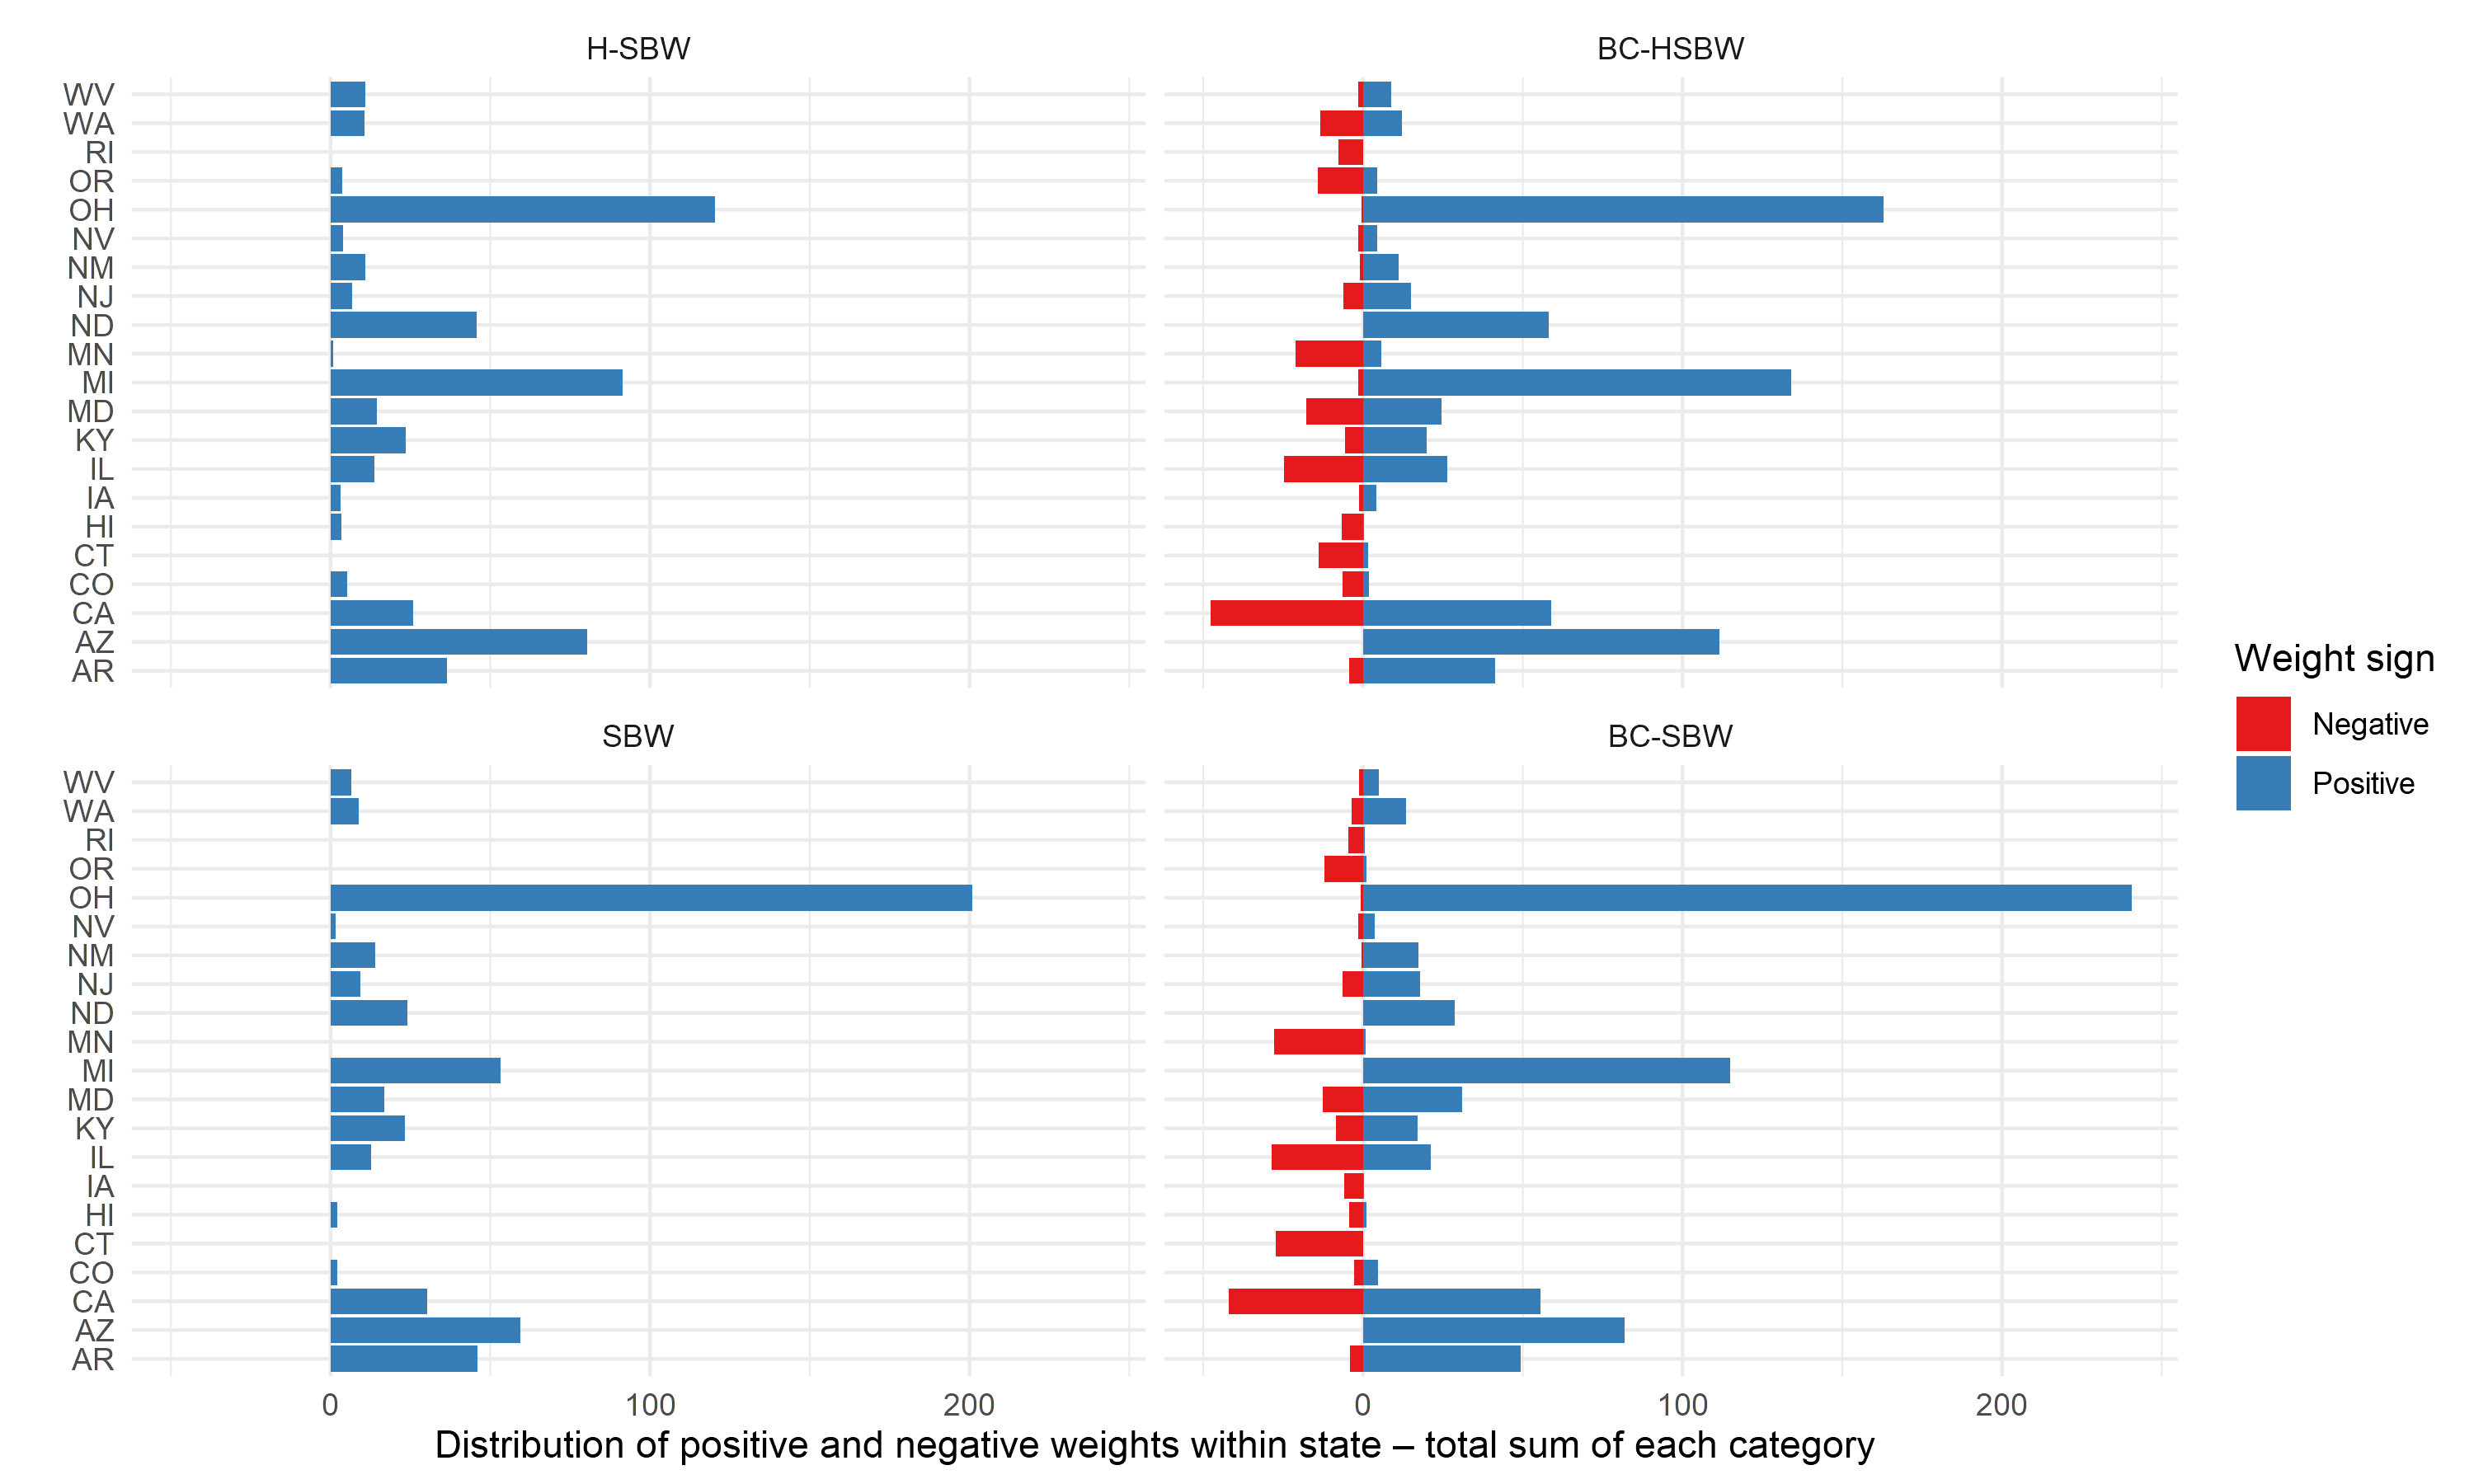
\includegraphics[scale=0.5]{01_Plots/weights-by-state-c1-all.png}
\end{center}
\end{figure}

\begin{figure}[H]
\begin{center}
    \caption{Total weights summed by state, early expansion excluded}
    \label{fig:weightsbystatec2all}
    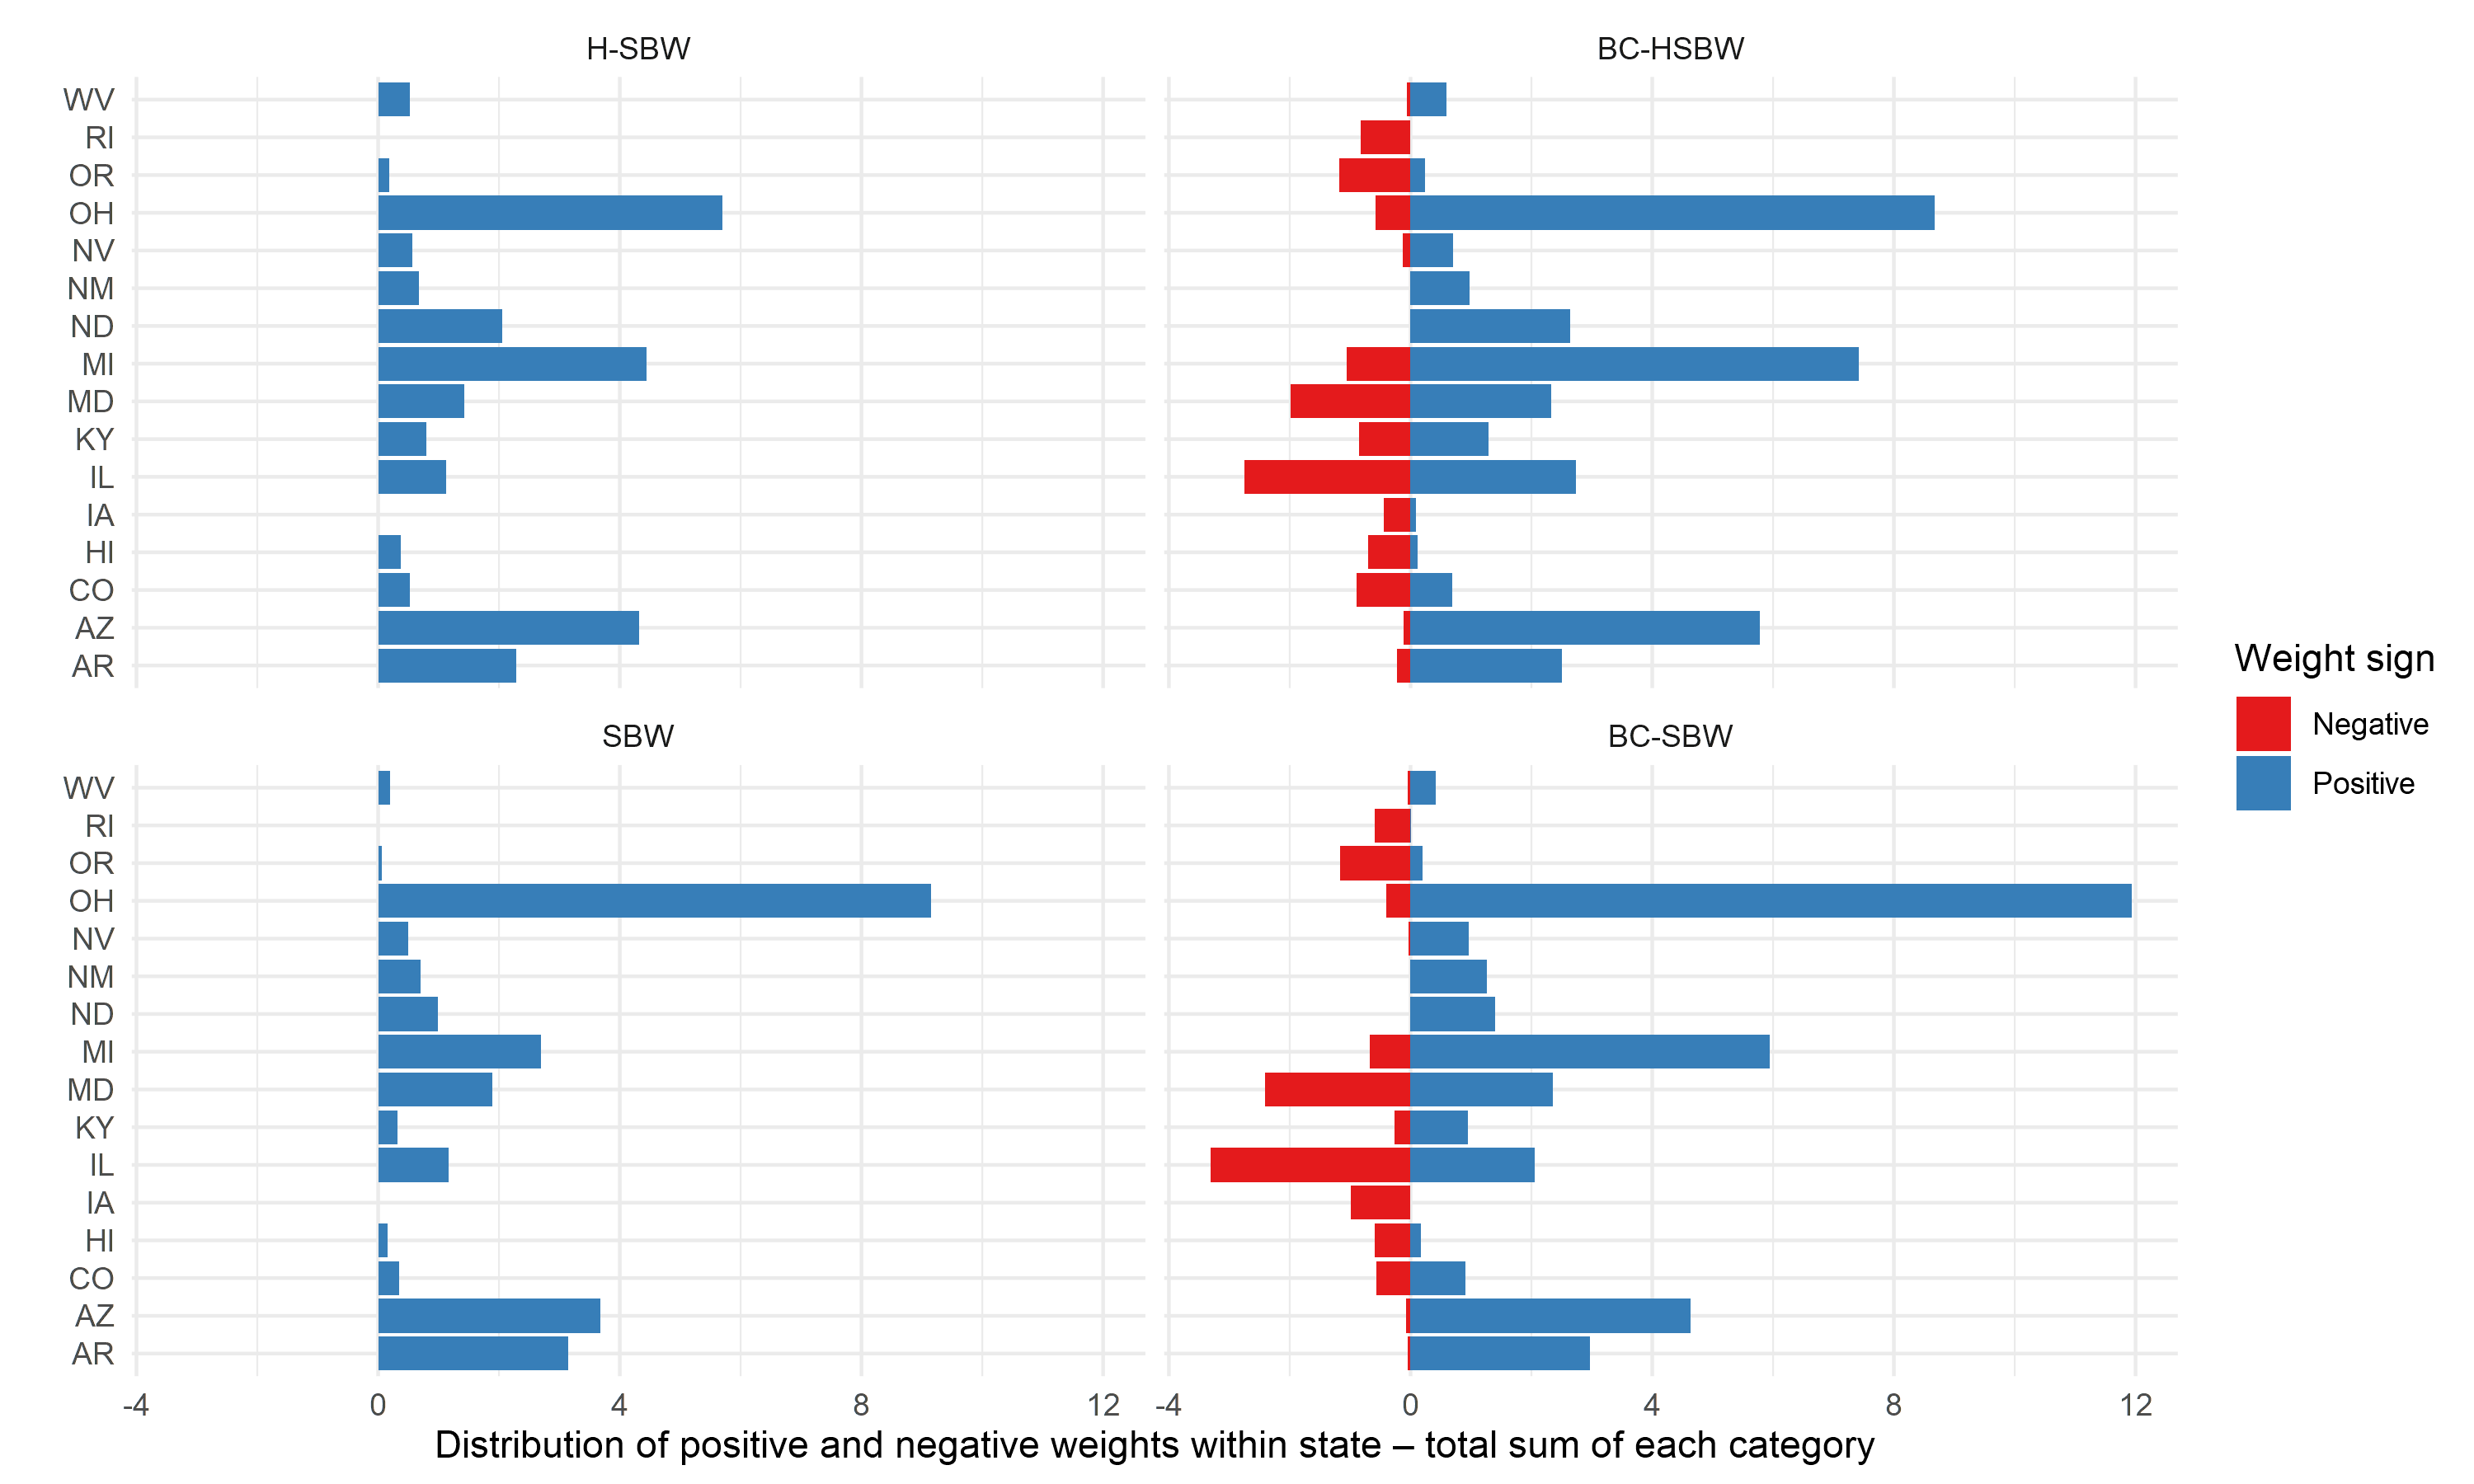
\includegraphics[scale=0.5]{01_Plots/weights-by-state-c2-all.png}
\end{center}
\end{figure}


\begin{table}[ht]
\caption{Balance comparison: weights estimated on unadjusted data applied to adjusted data}\label{tab:balcomp}
\begin{tabular}{lrrrr}
  \hline
Variables & Unweighted Diff & Weighted Difference & Homogeneous Diff & Heterogeneous Diff\\ 
  \hline
Uninsured Pct 2011 & -3.09 & -0.05 & -0.11 & 0.92 \\ 
  Uninsured Pct 2012 & -2.99 & -0.05 & -0.21 & -1.06 \\ 
  Uninsured Pct 2013 & -3.00 & -0.05 & -0.38 & -0.93 \\
  \hline
\end{tabular}
\end{table}
\clearpage